\section{Solution Overview} The solution which is inspired by similar work in the controls community \cite{mishra2017secure, chong2015observability} seeks to build a control framework for detecting attacks against UAVs. This is similar to using a program execution-invariant (such as runtime verification or Control Flow Integrity) to detect attacks on the compute subsystem. The control invariants are derived by using the physical attributes of the UAV (e.g, length of arm, weight etc.,), the underlying control algorithm used and the laws of physics. The controls invariant is used to formulate a normal behaviour of the vehicle as per the control input and the current physical state. Any deviation from this control invariant is used to raise a flag to indicate an anomaly.

The control invariant framework consists of three steps: 1) System Identification, 2) Controller Instrumentation, and 3) Formulating Anomaly Detection Statistics.

\subsection{System Identification} System identification is used to perform fitting of the UAV data according to the template of a linear time-invariant(LTI \footnote{While executing fast maneuvers, most UAVs are not linear systems. This assumption is for simplicity}) system as given in equations (1) and (2). This is done by running multiple missions and profiling the vehicle measurement data. From these measurements, values for matrices A, B, C and D are obtained. These form the invariant.  A key observation from CPS research \cite{shoukry2018smt, mishra2017secure}  is that UAVs having similar physical dimensions (e.g, all quadcopters) have the same control invariant template, only differing in the values of the coefficients A, B, C and D \cite{bouabdallah2004design}.

\begin{equation}
x_{k+1} = Ax_k + Bu_k
\end{equation}

\begin{equation}
y_k = Cx_k + Du_k
\end{equation}

From the laws of physics using Newton's laws of motion, we can derive the following two equations for a quadrotor \cite{bouabdallah2004design}. First is the equation in the linear acceleration along the frame of the earth as shown in Figure \ref{fig:linear}. Second is the equation of angular acceleration along the frame of the UAV as shown in Figure \ref{fig:angular}.


\begin{figure}
    \centering
    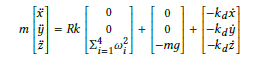
\includegraphics[scale=1.0]{images/linear.png}
    \caption{Equation describing linear physics of a quadrotor. m is the mass, $w_i$ the speed of the $i^{th}$ rotor, g the gravity, and R the conversion matrix from UAV frame to the inertial frame. $\dot{x}$, $\dot{y}$, $\dot{z}$ are velocities.The equation shows that the product of mass and acceleration is the sum of thrust, gravity and terminal drag force.}
    \label{fig:linear}
\end{figure}

\begin{figure}
    \centering
    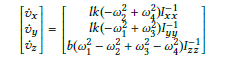
\includegraphics[scale=1.0]{images/angular.png}
    \caption{Equation describing angular physics of a quadrotor.This equation ties the rotational motion moment of inertia with the angular acceleration of the UAV. }
    \label{fig:angular}
\end{figure}

As a part of the template, we have a controller equation as well which in most cases, can be approximated by a PID controller. The PID controller is used to adjust the control signal (the rotor actuation currents) appropriately by monitoring the error. The PID controller takes into account the current error, the history of errors as well as the rate of change of the error. The equation for a PID contoller is shown in Figure \ref{fig:pid}.

\begin{figure}
    \centering
    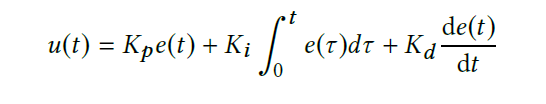
\includegraphics[scale=0.5]{images/pid.png}
    \caption{Equation describing PID controller used to approximate the controller in a UAV. }
    \label{fig:pid}
\end{figure}

We can measure the values of acceleration and velocities at different time-steps t and feed it into the PID controller to calculate the error calculated at different stages of flight.

The final stage of system identification is to use a System Identification tool in MATLAB to determine the values of unknown coefficients. As an illustration, using MATLAB, one is able to derive the values of A, B, C and D such as :

\begin{equation}
\resizebox{0.85 \hsize}{!}{
\left(\begin{array}{c} x(t+1) \\ y(t+1) \\z(t+1) \end{array}\right) = 
\left({\begin{array}{ccc} 0.7514 & -0.0565 & -0.0248 \\ 0.0758 & 0.9750 & 0.0075 \\ 0.0011 & 0.0025 & 0.9578 \end{array}}\right)
\left(\begin{array}{c} x(t) \\ y(t) \\ z(t) \end{array}\right)
+ 
\left(\begin{array}{c} 0.0078 \\ 0 \\ 0 \end{array}\right) 
\left(\begin{array}{c}external \  input \end{array}\right)
}
\end{equation}

\begin{equation}
\resizebox{0.85 \hsize}{!}{
\left(\begin{array}{c} Output \end{array}\right) = 
\begin{pmatrix} 1.2545 & 10.5876 & 10.0631 \end{pmatrix} 
\begin{pmatrix} x(t) \\ y(t) \\ z(t) \end{pmatrix}
+
\begin{pmatrix} 0.0025  \end{pmatrix} 
\left(\begin{array}{c}external \ input \end{array}\right)
}
\end{equation}


\begin{figure*}[h!]
    \centering
    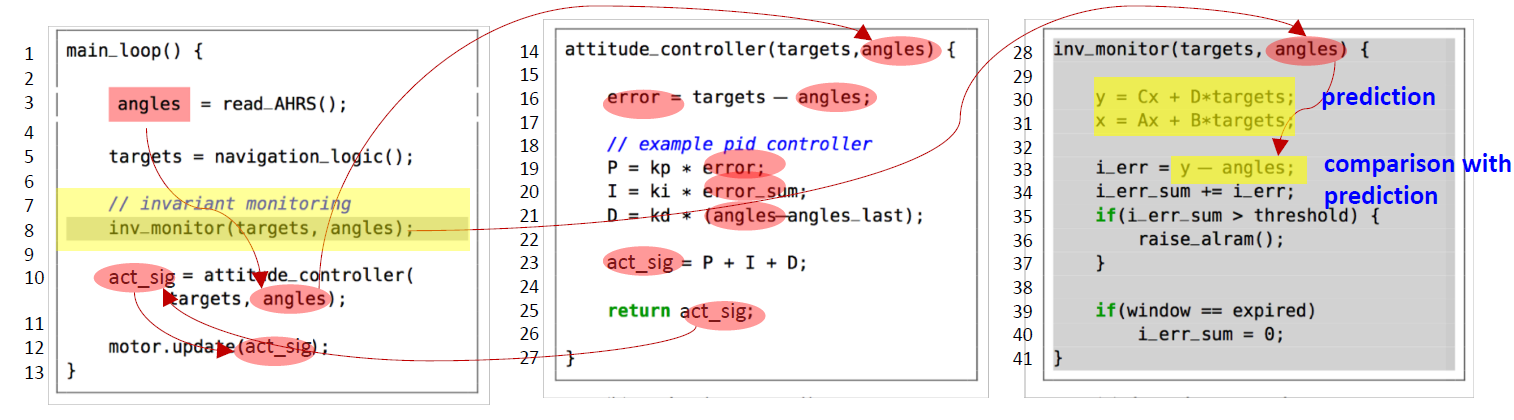
\includegraphics[width=\textwidth]{images/controller-invariant-framework.png}
    \caption{The propagation of false sensor values into the PID controller could potentially cause the UAV to undertake malicious navigation. Noting the error at various instances and comparing it with the actual value using the model can help avert this anomaly \cite{choi2018detecting}}
    \label{fig:controller-invariant-framework}
\end{figure*}

\subsection{Controller Instrumentation} The next step is to instrument the control loop inside the vehicle to take in the physical values of A, B, C and D that we have derived in the previous step. With this, one can then calculate the difference between the expected value (via the model) and the actual value as seen in practice, $d_k$. 

This step requires identifying those points in the autopilot code that corresponds to the physical parameter being output, such as the roll, pitch or the yaw angle. 


\subsection{Anomaly Detection Statistics} 
The squared error calculated can be then used to formulate a statistical test. Given a time series of values $d_k$, the anomaly detection test needs to determine when to raise an alarm. This could be done in two ways: In Stateless test, an alarm is raised for every single significant deviation at time k, i.e, if $d_k$ = |$y_k$ - $\hat{y}_k$| $\geq$ $\tau$, where $\tau$ is the threshold. In stateful test, there is an additional statistics $S_k$ to keep track of historical values of $d_k$, an generate an alert if $S_k$ $\geq$ $\tau$ i.e, if there is a persistent deviation across multiple time steps. Examples of tests used here include exponential moving average (EWMA) or a non-parametric cumulative sum statistic (CUSUM) \cite{healy1987note}.

A summary of the control invariant framework described is shown in Figure \ref{fig:controller-invariant-framework}


